\documentclass{scrartcl}

\usepackage{amsfonts}
\usepackage{amsmath}
\usepackage{multicol}
\usepackage{listings}
\usepackage{hyperref}
\usepackage{graphicx}
\hypersetup{
    colorlinks=true,
    linkcolor=blue,
    filecolor=magenta,      
    urlcolor=cyan,
    pdfpagemode=FullScreen,
}

\usepackage{xcolor}

\definecolor{mGreen}{rgb}{0,0.6,0}
\definecolor{mGray}{rgb}{0.5,0.5,0.5}
\definecolor{mPurple}{rgb}{0.58,0,0.82}
\definecolor{backgroundColour}{rgb}{0.95,0.95,0.92}

\lstdefinestyle{customc}{
  belowcaptionskip=1\baselineskip,
  breaklines=true,
  frame=L,
  xleftmargin=\parindent,
  language=C,
  showstringspaces=false,
  basicstyle=\footnotesize\ttfamily,
  keywordstyle=\bfseries\color{green!40!black},
  commentstyle=\itshape\color{purple!40!black},
  identifierstyle=\color{blue},
  stringstyle=\color{orange},
}

\lstdefinestyle{customasm}{
  belowcaptionskip=1\baselineskip,
  frame=L,
  xleftmargin=\parindent,
  language=[x86masm]Assembler,
  basicstyle=\footnotesize\ttfamily,
  commentstyle=\itshape\color{purple!40!black},
}

\lstset{escapechar=@,style=customc}

\usepackage{biblatex}
\addbibresource{biblography.bib}

\subject{GPU Computing}
\title{First Assignment - Report}
\author{
    Christian Dalvit\\
    {\small Student-ID: 249988}\\
    {\small E-mail: christian.dalvit@studenti.unitn.it}
}

\begin{document}
    \maketitle
    \thispagestyle{empty}
    \newpage

    \setcounter{page}{1}
    \section{Introduction}    
    The objective of this homework is to implement an algorithm for transposing a non-symmetric matrix and to measure and analyze various metrics of the algorithm. This report provides a description of the problem setting, algorithms, and experimental results of the implementation.
    The code used for this homework is made available through a public \href{https://github.com/chrisdalvit/matrix-transpose-benchmark}{Github repository}. Details on how to run the code and reproduce the results can be found in the \texttt{README.md} file of the Github repository.

    \section{Problem Description}
    For a given matrix $A \in \mathbb{R}^{n \times m}$, the transpose of the matrix $A^T \in \mathbb{R}^{m \times n}$ is defined as
    $$
        A^T_{ij} = A_{ji}
    $$
    In this homework, matrices have dimensions of $2^N$ for $N \in \mathbb{N}$, so only square matrices are considered. As a result, the implemented algorithms don't need to accommodate changes in the output matrix's shape. For the purpose of this homework, we assume a row-major memory layout of the matrix.
    While implementing an algorithm that computes the transpose of a matrix is straightforward, coming up with an efficient implementation is quite tricky. In general, leveraging spatial and temporal locality can improve efficiency. Because each element of the matrix is accessed only once, temporal locality cannot be exploited for computing the transposed matrix \cite{chatterjee2000cache}, so spatial locality becomes the only source for improvement. The issue with leveraging spatial locality in matrix transposition is that data is accessed along rows but written along columns, potentially leading to poor cache performance. Algorithms that respect spatial locality in their memory access pattern can benefit from quicker access to cached data. In the following, the different algorithms implemented during this homework are described and their memory access pattern is discussed.

    \subsection{Algorithms}
    In this homework, three different algorithms for in-place matrix transposition are implemented. Pseudocode for the algorithms can be found in the appendix. The first implementation, as shown in Figure \ref{fig:naive_implementation}, can be directly inferred from the mathematical definition. Transposition is performed by iterating over all entries above the matrix diagonal and swapping them with the corresponding entries below the diagonal. The first implementation will serve as the baseline implementation to measure performance improvements of other implementations. 
    The main issue with the naive implementation's memory access pattern is the disjointed access from \lstinline{mat[j*size+i]}, potentially causing poor cache performance, especially with larger matrices where \lstinline{mat[j*size+i]} might not be present in cache and requires loading from memory.

    The second implementation (Figure \ref{fig:prefetch_implementation}) tries to improve performance by prefetching the memory addresses needed in the next iteration. This should reduce cache-miss latency by moving data into the cache before it is accessed \cite{gccdocs}. The built-in function \lstinline{__builtin_prefetch} can be used to perform prefetching. \lstinline{__builtin_prefetch} takes as arguments the address to be prefetched and two optional arguments \textit{rw} and \textit{locality}. Setting \textit{rw} to $1$ means preparing the prefetch for write access and setting \textit{locality} to $1$ means that the prefetched data has low temporal locality \cite{gccdocs}. The second implementation is referred to as ``prefetch''-implementation.

    The third algorithm (Figure \ref{fig:rec_implementation}) implements a recursive pattern for matrix transposition. It uses the fact that 
    \begin{equation*}
        \begin{pmatrix}
            A & B \\
            C & D
        \end{pmatrix}^T = 
        \begin{pmatrix}
            A^T & C^T \\
            B^T & D^T
        \end{pmatrix}
    \end{equation*}
    Where $A, B, C$ and $D$ are submatrices. Note that the submatrices $B$ and $C$ get swapped. The idea behind this algorithm is that it splits the matrix into four sub-matrices until the submatrices fit into the cache. Then the submatrices get transposed and the quadrants get swapped. Figure \ref{fig:rec_implementation} depicts pseudocode for this algorithm. For a matrix size of 128 or smaller the algorithm performs a normal transpose operation (i.e. the \lstinline{swap_small_matrix}-function call in Figure \ref{fig:rec_implementation}). Otherwise, the matrix is split into four submatrices and the function is called recursively (i.e. the \lstinline{else}-block in Figure \ref{fig:rec_implementation}). After the transposition of the submatrices, the upper-right and bottom-left quadrants need to be swapped (i.e. the \lstinline{swap_quadrants}-function call in Figure \ref{fig:rec_implementation}).\\
    This algorithm exploits spatial locality as it divides the matrix into sub-matrices that can fit into the cache. The third algorithm also has a reduced I/O complexity of $\mathcal{O}(\frac{N^2}{B})$ \cite{algorithmica}, where $N$ is the size of the matrix and $B$ the size of the blocks (i.e. the size of matrices where standard transposition is performed). It then transposes each submatrix, which can be performed more efficiently as the whole submatrix is present in cache. This algorithm also works quite well for large matrices, because they are always reduced to submatrices of sizes that fit into cache. The threshold of 128 for performing standard matrix transposition, was selected because the MacBook Air has an L1 data cache of 65KB (as described in Section \ref{sec:experiments}). Since each matrix element is an integer having a size of $4$ bytes, a submatrix of dimension 128 needs $128*128*4 = 65536$ bytes. Therefore one submatrix fits in the L1 data cache, which should result in better performance. During the homework, the same algorithm was tested for threshold values 32, 64, 128, 256 and 512. The results indicated that the algorithm performed best with a threshold of 128 on the tested architectures.

    \section{Experiments} \label{sec:experiments}
    \subsection{Setup}
    The three algorithms were implemented in C. Each algorithm was compiled with optimization levels \texttt{-O0}, \texttt{-O1}, \texttt{-O2}, \texttt{-O3}. Each resulting binary was evaluated 50 times for matrix sizes between $2^8$ and $2^{14}$. Cache data was collected using Valgrind \cite{valgrind}. Each binary was benchmarked with the Cachegrind tool for matrix size $2^{14}$. The experiments were conducted on two different architectures
    \begin{itemize}
        \item MacBook Air (2020) having a M1 chip with 3,2 GHz and 8 cores, 8GB of RAM, 131KB L1 instruction cache, 65KB L1 data cache, 4.2 MB L2 cache and a cacheline size of 128 byte.
        \item iMac (2011) having a Intel Core i5 with 2.5GHz and 4 cores, 8GB of RAM, 64KB L1 cache, 1MB L2 cache, 6MB L3 cache and a cacheline size of 64 byte.
    \end{itemize}
    Unfortunately Valgrind is not officially supported for ARM-based Apple computers \cite{valgrinddocs} and Open-Source projects working on compatibility for M1 processors are still in the experimental phase \cite{valgrindm1bug}. Therefore it is not possible to provide cache performance data for the MacBook Air experiments. 

    \subsection{Results}    
    The execution times of the different algorithms are compared in Figure \ref{fig:time_comparison}.
    The third algorithm (\texttt{oblivious128} in Figure \ref{fig:time_comparison}) achieved the highest speedup with optimization flags. It showed a speedup of $7.81$ on the MacBook Air and $5.7$ on the iMac when comparing non-optimized code to code with \texttt{-O3} enabled for matrix size $2^{14}$.
    On the MacBook Air, the third algorithm gained an additional speedup of $1.46$ for matrix size $2^{14}$ using \texttt{-O2} and \texttt{-O3} optimizations compared to \texttt{-O1} optimization.
    The second algorithm (\texttt{naive\_prefetch} in Figure \ref{fig:time_comparison}) performs slightly better for large matrices with some optimization enabled, resulting in a speedup of $2.11$ on the MacBook Air and $1.73$ on the iMac for matrix size $2^{14}$.
    Enabling optimization flags can be disadvantageous for execution time performance (see \texttt{naive} and \texttt{naive\_prefetch} implementations for matrix size $2^{10}$).
    \begin{figure}
        \begin{center}
            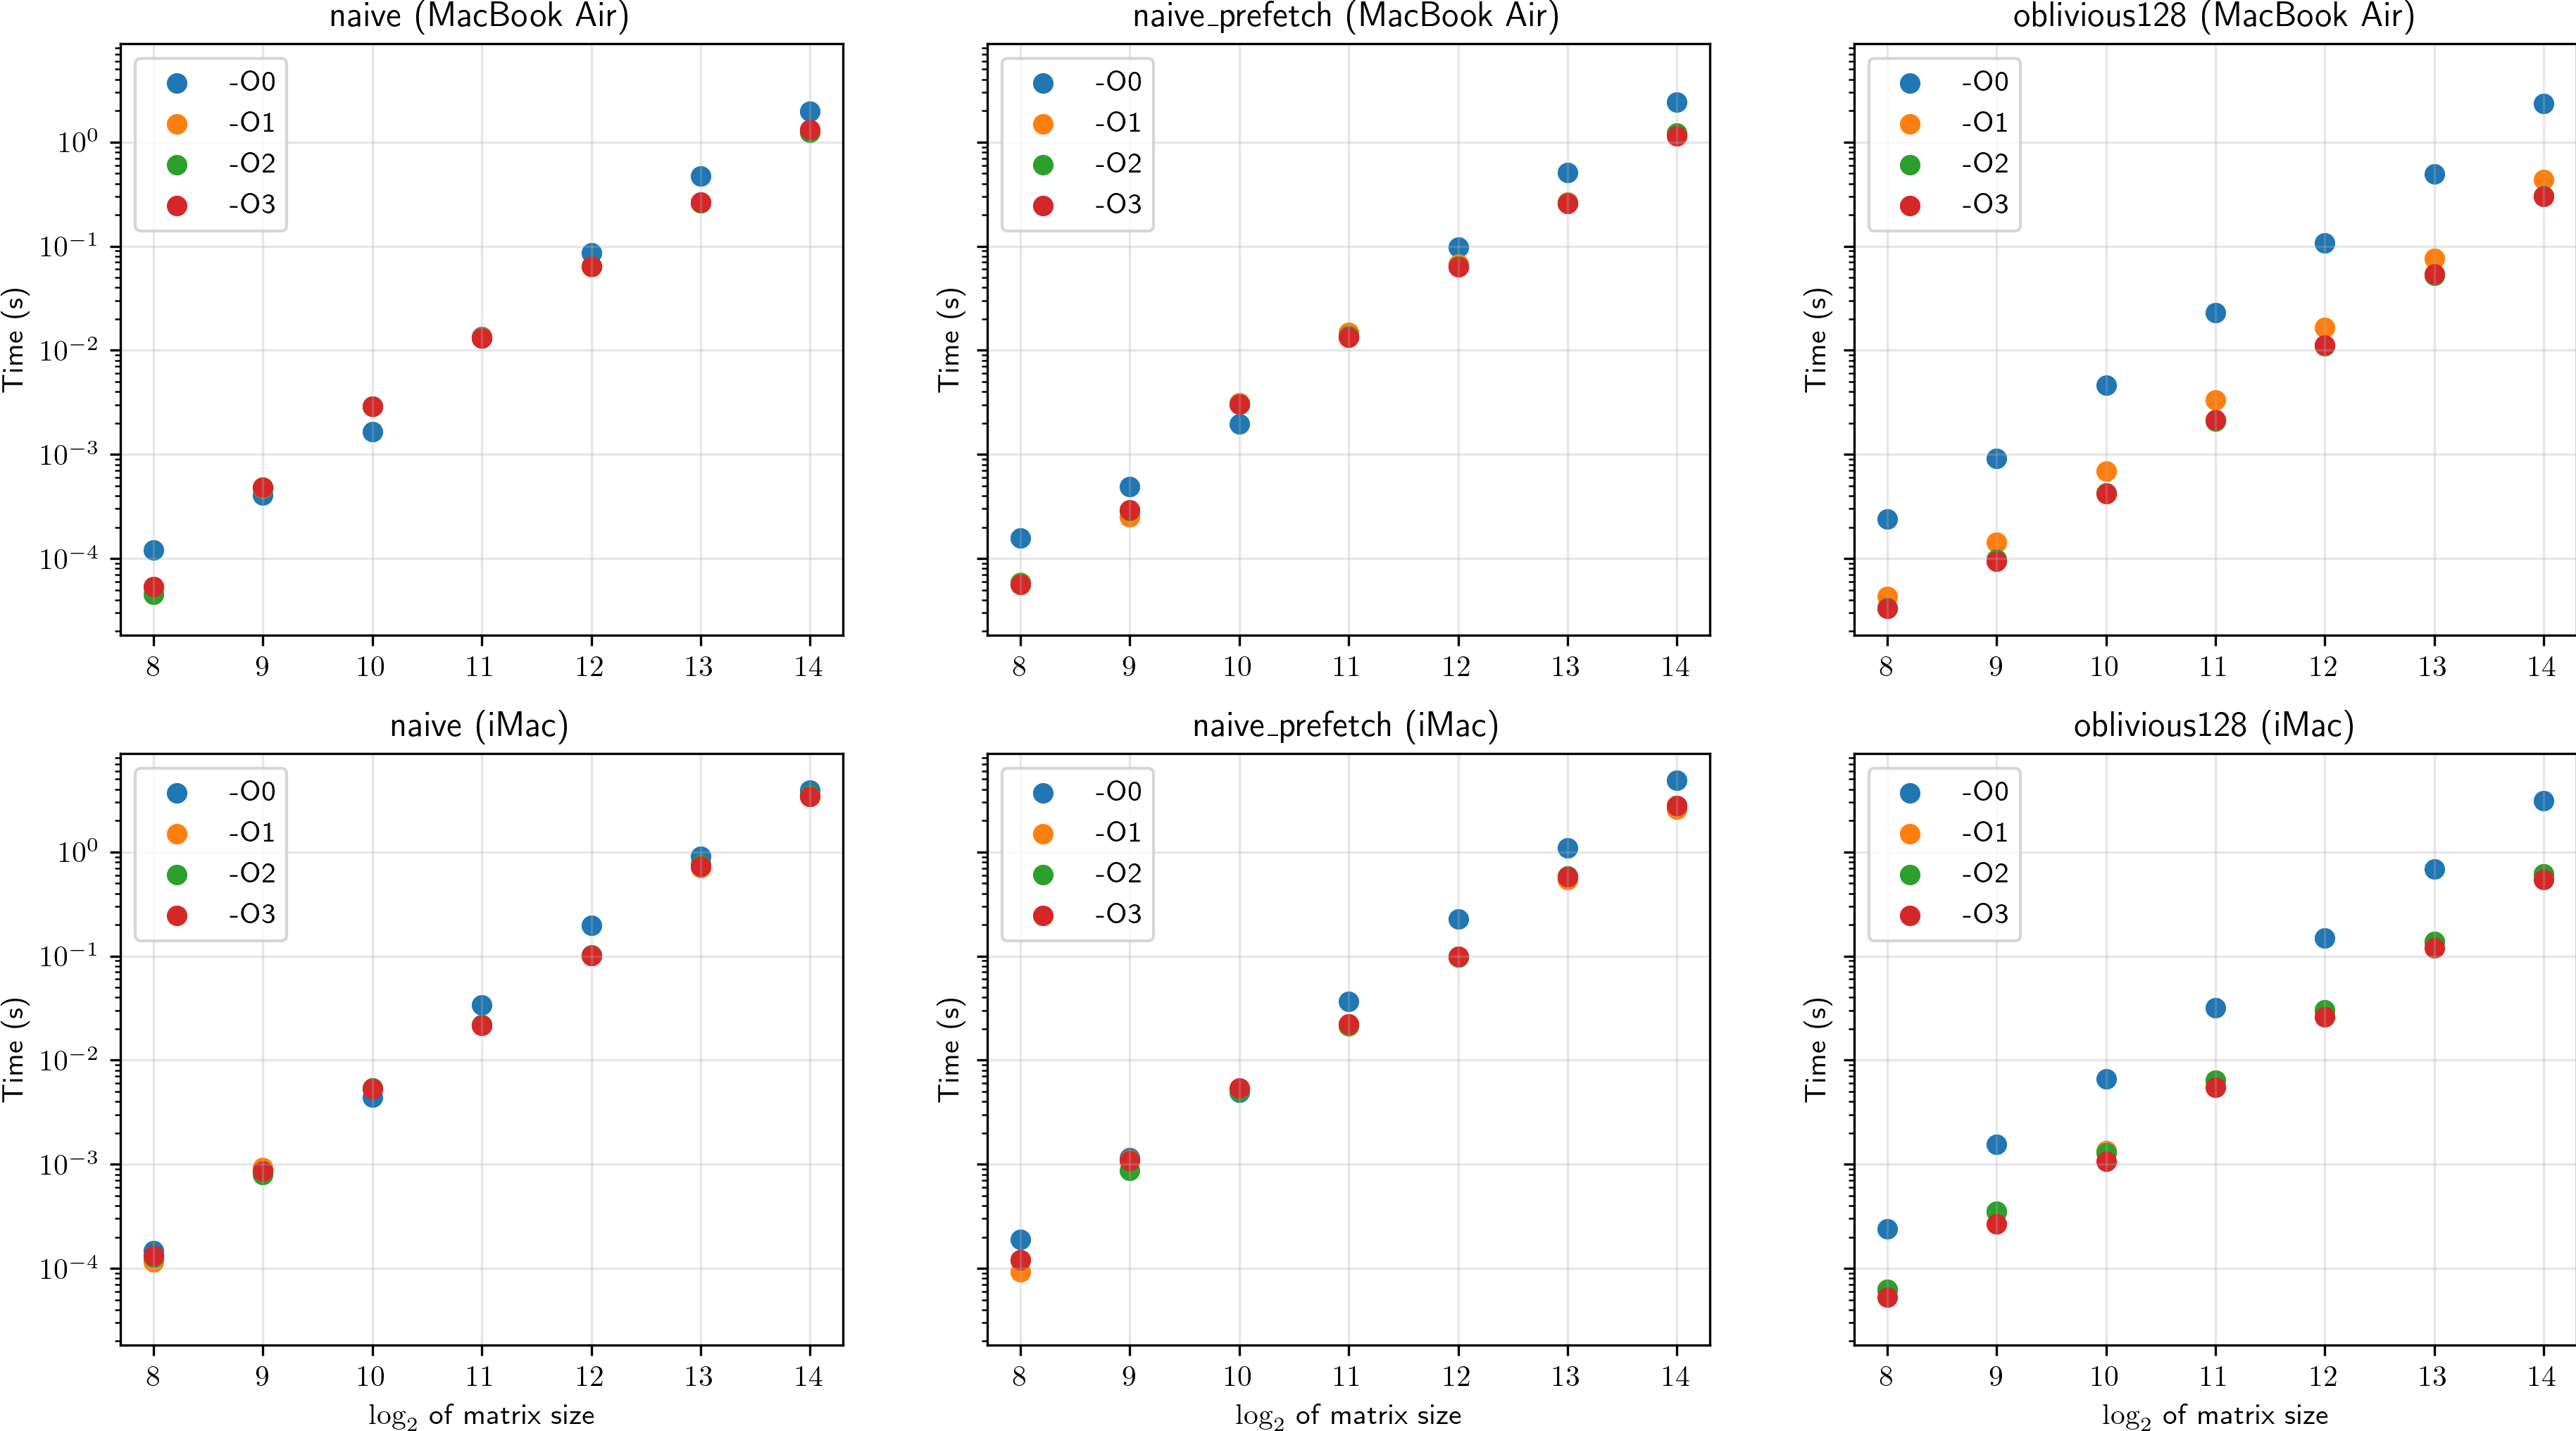
\includegraphics[width=0.6\textwidth]{./images/time_comparision.png}
        \end{center}
        \caption{Comparison of the mean execution time of various algorithms for matrix sizes ranging from $2^8$ to $2^{14}$ for the MacBook Air architecture (upper row) and iMac architecture (bottom row). The y-axis denotes the execution time in seconds and is depicted on a logarithmic scale.}
        \label{fig:time_comparison}  
    \end{figure}
    The effective bandwidth of the different algorithms is compared in Figure \ref{fig:bandwidth_comparison}. It's evident across all graphs that the effective bandwidth decreases as the matrix size increases. This trend arises because the matrix size grows exponentially with a base of $2$, while the execution time grows exponentially with a base of roughly $10$, as illustrated in Figure \ref{fig:time_comparison}. Consequently, the execution time increases more rapidly than the matrix size, leading to a decline in effective bandwidth.
    \begin{figure}
        \begin{center}
            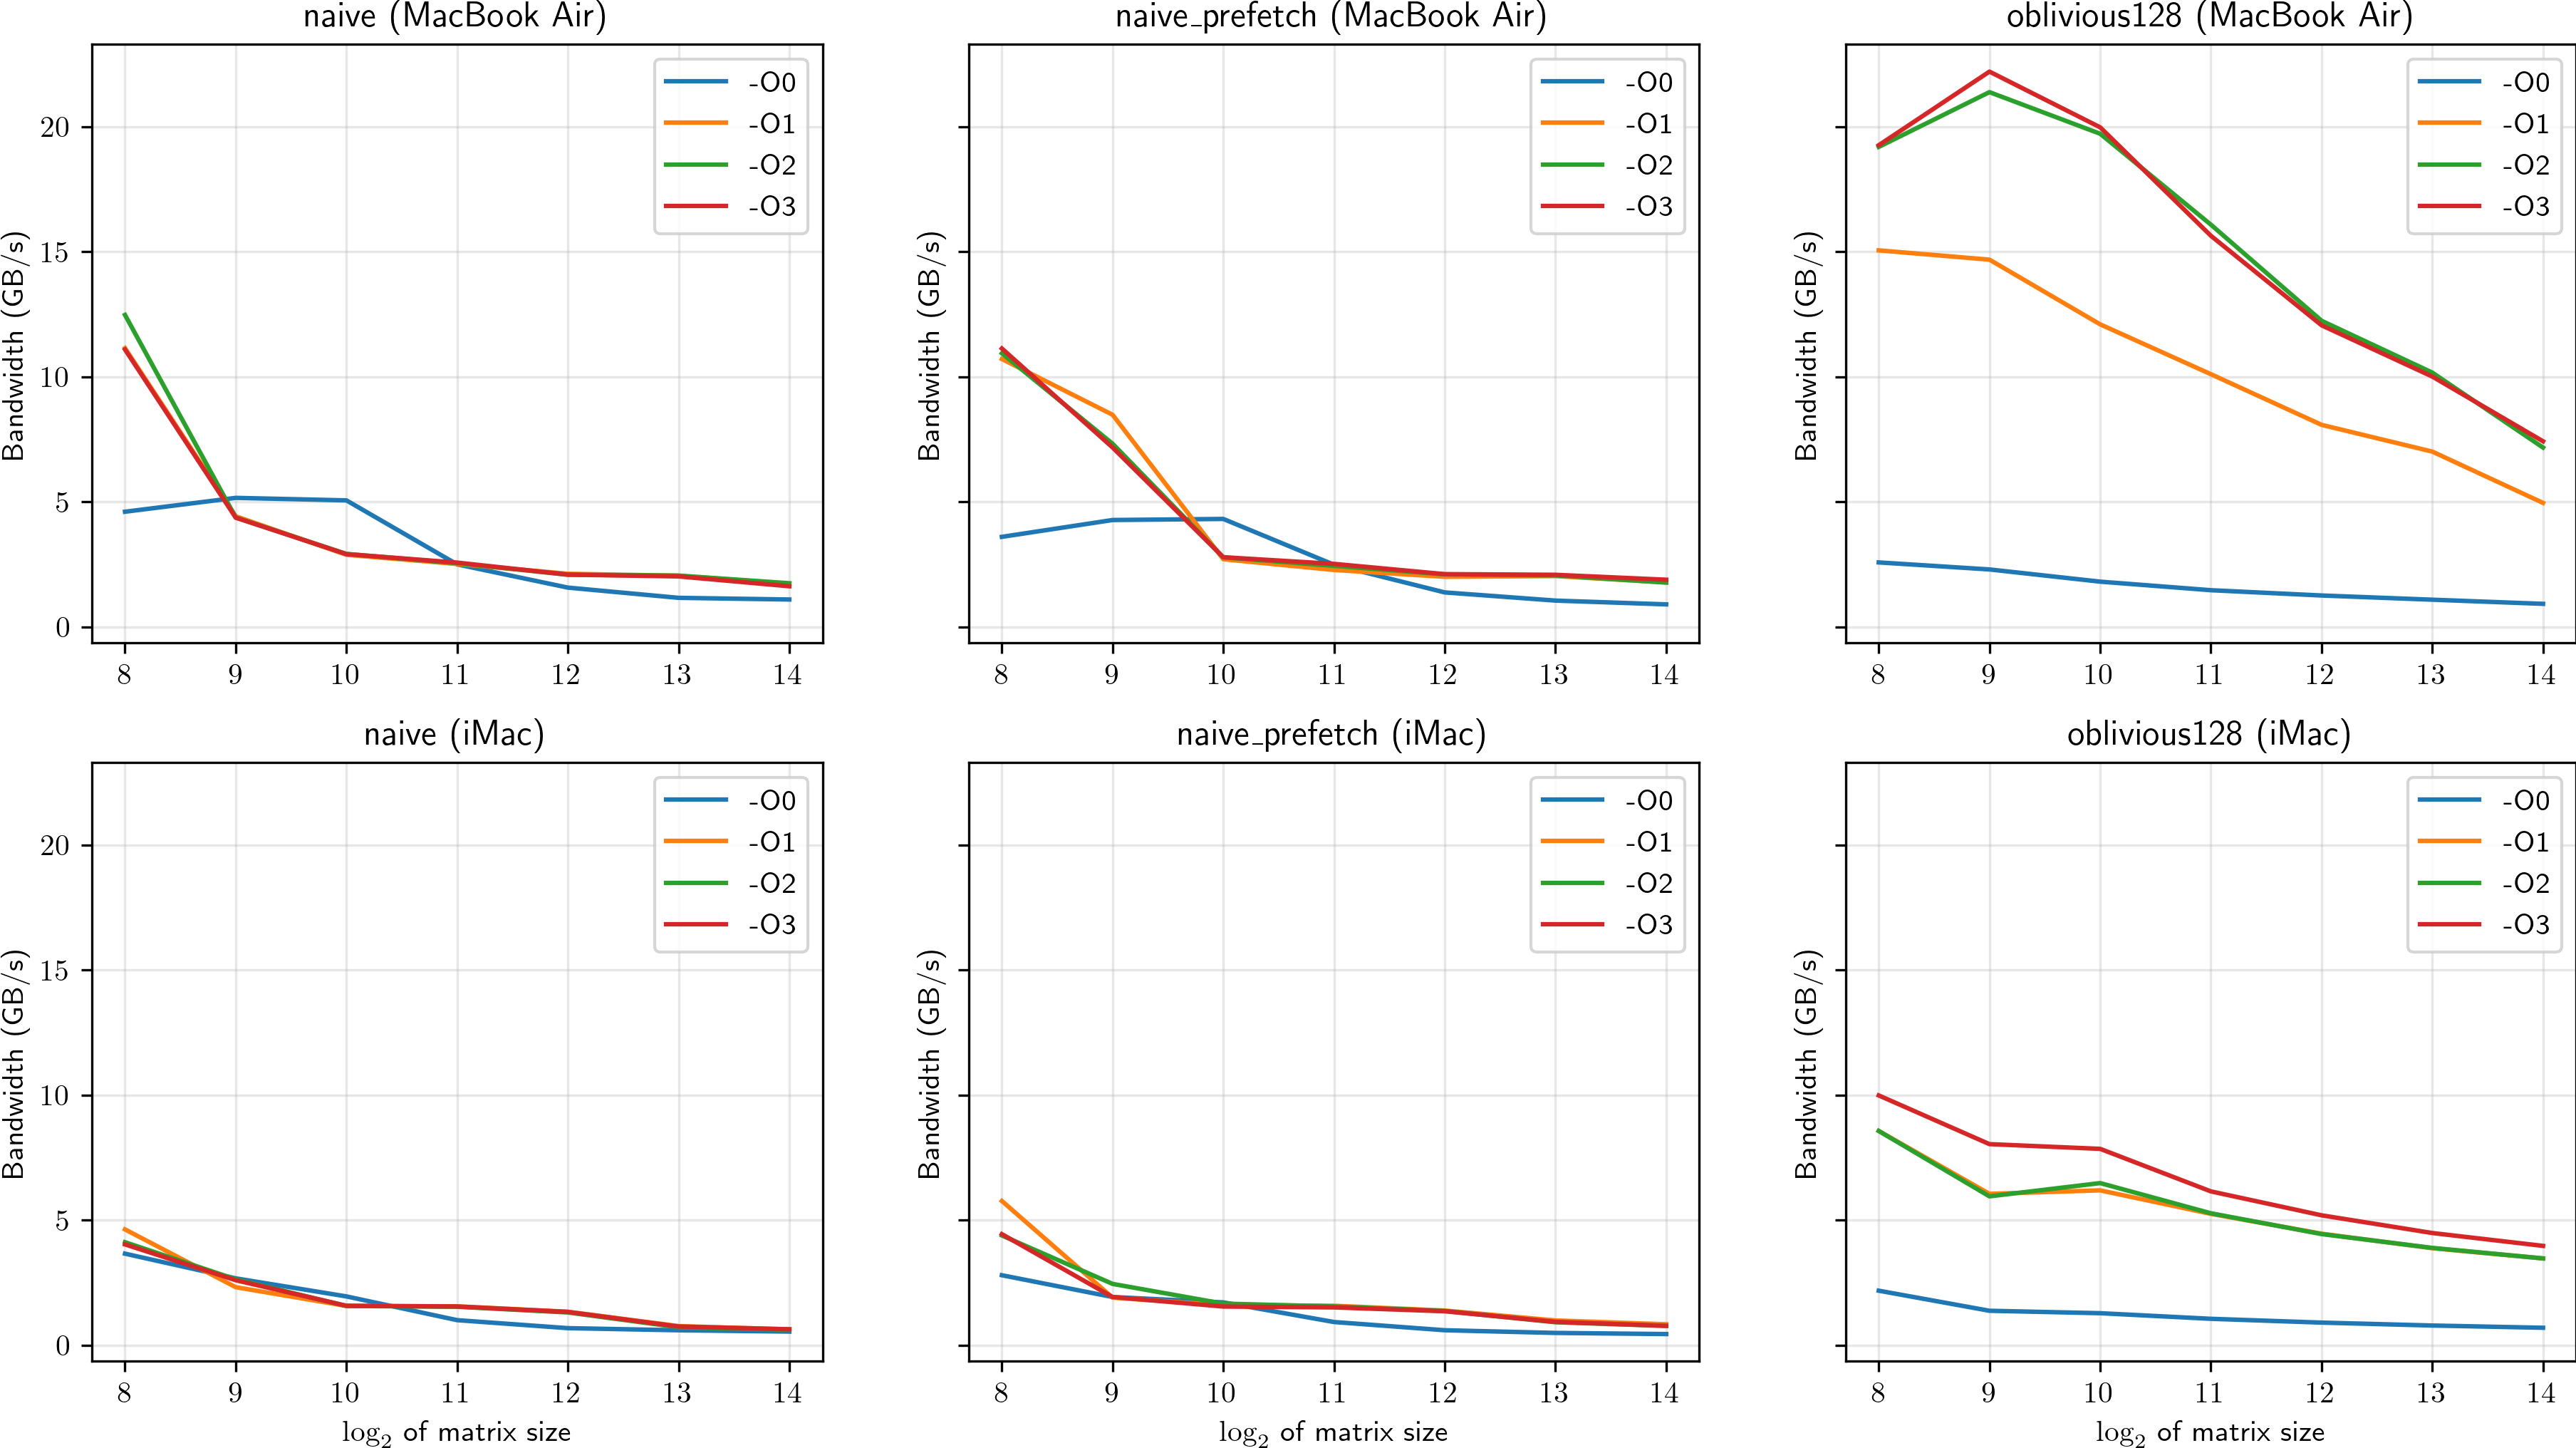
\includegraphics[width=0.6\textwidth]{./images/bandwidth_comparision.png}
        \end{center}
        \caption{Comparison of the mean effective bandwidth of different algorithms for matrix sizes between $2^8$ and $2^{14}$ for the MacBook Air architecture (upper row) and iMac architecture (bottom row).}
        \label{fig:bandwidth_comparison}  
    \end{figure}
    Cache data, as depicted in Figure \ref{tab:cache_data} in the appendix, reveals distinctive behaviors among implementations. Specifically, the \texttt{naive} and \texttt{naive\_prefetch} implementations show similar cache patterns, while the \texttt{oblivious128} implementation stands out with different cache behavior. Comparing cache data across implementations, it's evident that the \texttt{oblivious128} implementation requires approximately twice as many instructions, data reads, and data writes as the \texttt{naive} implementation. The variance could be a result of the extra instructions required for transposing submatrices and copying quadrants in the \texttt{oblivious128} algorithm, leading to a greater overall instruction count. Another notable finding is that the last-level data cache read misses are significantly lower for the \texttt{oblivious128} implementation. This may be due to the improved fit of submatrices utilized in the \texttt{oblivious128} algorithm within the cache.

    \section{Conclusion}
    After analyzing various algorithms and metrics, it's evident that utilizing blocks can enhance the performance of matrix transposition algorithms. This was demonstrated through the better execution time and effective bandwidth of compiler-optimized versions of the \texttt{oblivious128} implementation, which incorporates a form of blocking. The third algorithm also presents promising directions for parallelization, as each submatrix can be processed independently, offering straightforward potential for parallel execution.

    \newpage
    \printbibliography

    \appendix
    \section{Pseudocode}

    \begin{figure}[h!]
        \begin{lstlisting}[language=C]
            void naive_transpose(int size, int* mat){
                for(int i = 0; i < size; i++){
                    for(int j = i+1; j < size; j++){
                        swap(mat[i*size+j], mat[j*size+i]);
                    }
                }
            }
        \end{lstlisting}
        \caption{Pseudocode for the naive implementation.}
        \label{fig:naive_implementation}        
    \end{figure}

    \begin{figure}[h!]
        \begin{lstlisting}[language=C]
            void prefetch_transpose(int size, int* mat){
                for(int i = 0; i < size; i++){
                    for(int j = i+1; j < size; j++){
                        swap(mat[i*size+j], mat[j*size+i]);
                        __builtin_prefetch(&mat[j*size+(i+1)], 0, 1);
                        __builtin_prefetch(&mat[(i+1)*size+j], 1, 1);
                    }
                }
            }
        \end{lstlisting}
        \caption{Pseudocode for the naive implementation with prefetch.}
        \label{fig:prefetch_implementation}        
    \end{figure}

    \begin{figure}[h!]
        \begin{lstlisting}[language=C]
            void transpose_block(int size, int *mat, int row_offset, int col_offset) {
                if (size <= 128) {
                    swap_small_matrix(size, mat, row_offset, col_offset);
                } else {
                    int m = size / 2;
                    transpose_block(m, mat, row_offset, col_offset);
                    transpose_block(m, mat, row_offset, col_offset+m);
                    transpose_block(m, mat, row_offset+m, col_offset);
                    transpose_block(m, mat, row_offset+m, col_offset+m);
            
                    // Swap upper-right and bottom-left quadrants
                    swap_quadrants(m, mat, row_offset, col_offset);
                }
            }
        \end{lstlisting}
        \caption{Naive implementation with prefetch of in-place matrix transposition.}
        \label{fig:rec_implementation}        
    \end{figure}

    \begin{figure}[h!]
        \begin{center}
            \begin{tabular}{ | c | c | c | c | c | c | c |}
                \hline  
                Name                    & Ir    & Dr    & DLmr  & Dw    & D1mw  & DLmw \\
                \hline  
                \texttt{naive}          & 20.6  & 5.1   & 0.14  & 2.4   & 0.016 & 0.016\\ 
                \hline  
                \texttt{oblivious128}   & 41.1  & 10.1  & 0.041 & 4.7   & 0.033 & 0.033\\      
                \hline  
            \end{tabular}            
        \end{center}
        \caption{Summarized cache data for different implementations with \texttt{-O3} optimization. Values are given in billions.}
        \label{tab:cache_data}
    \end{figure}

\end{document}